\documentclass{article}

\usepackage[a4paper, total={6in, 9in}]{geometry}


\usepackage[utf8]{inputenc}
\usepackage{amsmath}
\usepackage{amsfonts}
\usepackage{amssymb}

\usepackage{amsthm}
\usepackage{french}

\usepackage{graphicx}

\input{insbox}

\usepackage{hyperref}
\hypersetup{
    colorlinks=true,
    linkcolor=blue,
    filecolor=magenta,      
    urlcolor=cyan,
}

\begin{document}

\section{La Théorie}

\subsubsection{Tableau de données}

L'Analyse en Composante Pricipale s'interesse à l'etude des tableaux de données rectangulaires dont les lignes sont appelées \textit{Individus} et les colonnes sont appelées \textit{Variables}.
\newline

L'image ci-dessous illustre un tableau de donnees a \textit{n-individus} et a \textit{p-variables}. Un \textit{individu} est noté $i=(x_{i1},x_{i2}, ... ,x_{ip}) \in \mathbb{R}^p$ et une \textit{variable} est notée $x_j=(x_{1j},x_{2j}, ... ,x_{nj}) \in \mathbb{R}^n$
\newline

\underline{NB:} Il est important de souligner que les \textit{variables} sont \textbf{quantitatives} en ACP, c'est à dire que $x_{ij} \in \mathbb{R}, \; \forall (i,j) \in [n]\times[p].$

\begin{figure}[h!]
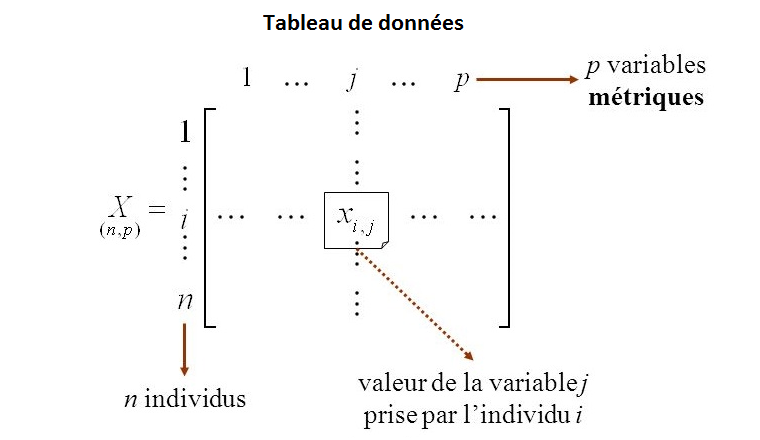
\includegraphics[width=\linewidth]{images/tableau.png}
\end{figure}

\subsubsection{Moyenne et Variance}

Pour une \textit{variable} ${x_j}$, on note sa moyenne $\bar{x}_j$ et son écart-type $s_j$ telles que:

\begin{equation*}
\bar{x}_j=\frac{1}{n}\sum_{i=1}^{n}{x_{ij}} \;\;\;\;\;\;\;\;\;\; s_j=\sqrt{\frac{1}{n}\sum_{i=1}^{n}{(x_{ij}-\bar{x}_j)^2}}
\end{equation*}

\subsubsection{Distance et Point moyen}
En ACP, il est important de savoir quels \textit{individus} sont proches les un des autres, pour pouvoir, si possible, creer des groupes d'\textit{individus} selon leur proximité. Il est alors necessaire de definir une distance entre deux \textit{individus} i et i', soit d cette distance:

\begin{equation*}
d^2(i,i')=\sum_{j=1}^{p}{(x_{ij}-x_{i'j})^2} 
\end{equation*}

\newpage

De plus, à partir de la moyenne de chaque \textit{variables}, on construit un point noté G et appelé \textbf{point moyen} du nuage des \textit{individus}, ce point peut etre interpreté comme le centre de gravité du nuage des \textit{individus}:

\begin{equation*}
G=(\bar{x}_1,\bar{x}_2,...,\bar{x}_p)
\end{equation*}

\subsubsection{Centrage et Réduction}
Ayant le point moyen, qui peut être vue comme le centre de gravité du nuage, il est conseillé de translater notre nuage de telle façon que G soit confondue avec le centre du repère, cela ce traduit par: ``Replacer $x_j$ par $x_{ij}-\bar{x}_j$ dans le tableau de données'';
\newline

Cette processus s'appelle \textbf{centrage} et elle améliore grandement l'affichage et l'interprétation des graphiques de nos données.

\begin{equation*}
x_{ij} \leftarrow x_{ij}-\bar{x}_j \;\;\;\;\; \forall i \in [n], \; \forall j \in [p],
\end{equation*}
\newline

Parfois, les \textit{variables} ne sont du même unité, ceci peut entrainer une ambiguïté dans l'interprétation des données, en effet, une variable a une ``quantité'' plus petite, dans le tableau, lorsqu'elle est exprimé en mettre, que lorsqu'elle est exprimé en centimètre. Ce qui peut entrainer, respectivement aux unités, une faible ou une forte importance par rapport aux autres variables qui faussera alors l'analyse.
\newline

Un moyen efficace d'eviter ce probleme est la \textbf{reduction}, elle consiste a diviser les \textit{variables} par leur écart-type.
\newline

Comme on a convenu plutot qu'il est preferable de centrer les \textit{variables}, alors le \textbf{centrage} et la \textbf{reduction} se traduit par: ``Replacer $x_j$ par $(x_{ij}-\bar{x}_j)/s_j$ dans le tableau de données'';

\begin{equation*}
x_{ij} \leftarrow \frac{x_{ij}-\bar{x}_j}{s_j}  \;\;\;\;\; \forall i \in [n], \; \forall j \in [p]
\end{equation*}
\newline

\underline{NB:} Apres le centrage et la reduction, nos nouvelles \textit{variables} sont alors ``asymptotiquement'' de moyenne nulle et de variance egale a un. c'est a dire:

\begin{equation*}
\bar{x}_j \approx 0 \;\;\;\;\; s_j^2 \approx 1 \;\;\;\;\; \forall j \in [p]
\end{equation*}

\subsubsection{Inertie}

Par definition, l'inertie \textit{I} des données est:

\begin{equation*}
I = \frac{1}{n} \sum_{i=1}^n \sum_{j=1}^p {\left( \frac{x_{ij}-\bar{x}_j}{s_j} \right)}^2
\end{equation*}

C'est donc, au coefficient 1/n pres, la somme des carrés de toutes les cellules du tableau de données apres centrage et reduction, mais elle peut egalement etre interpretée par rapport aux \textit{individus} et aux \textit{variables}.

\newpage

\begin{flushleft}
\textbf{Inertie et Individus}
\end{flushleft}

Soit l'individu $i \in [n]$, la quantité $\sum_{j=1}^p {\left( \frac{x_{ij}-\bar{x}_j}{s_j} \right)}^2$ de l'inertie represente la distance entre cet individue et le point moyen G. Par conséquent, l’inertie peut etre vue comme la somme des carres des distances au centre de gravite pour tous les individus.
\newline

Ainsi, l’inertie renseigne sur la ``forme'' du nuage des individus. En effet, plus la distance entre les individus sont grande (resp. petite), plus l'inertie est grande (resp. petite).

\begin{flushleft}
\textbf{Inertie et Variables}
\end{flushleft}

Dans la definition de l'inertie, les deux somme $\sum$ peuvent etre interverti, ainsi, on a une autre expression:

\begin{equation*}
I = \frac{1}{n} \sum_{j=1}^p \sum_{i=1}^n {\left( \frac{x_{ij}-\bar{x}_j}{s_j} \right)}^2
\end{equation*}

Ici, on peut remarquer que la quantité $\sum_{i=1}^n {\left( \frac{x_{ij}-\bar{x}_j}{s_j} \right)}^2$ correspond au carré de la norme de la variable centrée reduite $x_j$ ou $j \in [p]$. Or cette quantité est egale à n, ainsi, l'inertie est toujour egale au nombre de variables, en effet:

\begin{align*}
I &= \frac{1}{n} \sum_{j=1}^p \sum_{i=1}^n {\left( \frac{x_{ij}-\bar{x}_j}{s_j} \right)}^2 \\
  &= \frac{1}{n} \sum_{j=1}^p \left( \frac{1}{s_j^2} \; n{s_j^2} \right) \\  
  &= \frac{1}{n} \sum_{j=1}^p \left( \frac{1}{s_j^2} \; n{s_j^2} \right) \\
  &= \frac{1}{n} \sum_{j=1}^p n \\
  &= \frac{1}{n} \; pn \\
  &= p
\end{align*}
\\

\subsubsection{Représentation Simplifiée}

On a vu que les \textit{variables} sont des vecteurs de $\mathbb{R}^p$, alors, quand $p > 3$, il n'est plus possible de representer les variables. L'ACP vise a fournir une image simplifiée du nuage des \textit{individus} la plus fidele possible, cest a dire, trouver une sous-espace de dimension plus petite qui resume au mieux les données.
\newline

\newpage

\begin{flushleft}
\textbf{Comment retrouver la meilleur sous-espace?}
\end{flushleft}

Pensons pour cela a l’image d’un chameau, la figure ci-dessous propose deux
representations simplifiees de cette image: des representations en dimension 2, la vue de face et la vue de profil.

\begin{figure}[h!]
\centering
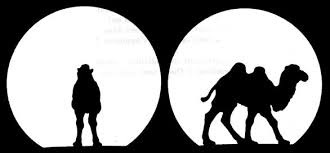
\includegraphics[width=200px]{images/chameau.png}
\end{figure}

Il est evident de dire que la meilleure representation simplifiee est la vue de profil. La raison est que l’image projetee du chameau dans ce plan est plus proche de l’image initiale dans le sens ou la variabilite des points qui la representent est plus grande et donc restitue mieux la variabilitee des points d’origine en dimension 3.
\newline

On a alors les etapes suivantes pour retouver analytiquement la meilleure representation simplifiee du nuage des \textit{individus}:

\begin{flushleft}
Etape 1: \textbf{Trouver l'axe qui deforme le moins possible le nuage}
\end{flushleft}

On cherche un axe dans $\mathbb{R}^p$ de sorte que les distances entre les points initiaux i (\textit{individu}) soient les plus proches possibles de leurs projetes orthogonaux sur cette axe et cela en tenant compte de tous les autres points. Notons $\vec{u}_1$ la direction de cet axe, et $H_i$ la projetée orthogonale de i.
\newline

\InsertBoxL{0}{\quad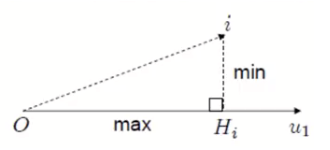
\includegraphics[width=200px]{images/projection.png}\quad} %

Le but est de minimiser la distance $iH_i$, ce qui revient a maximiser la distance $OH_i$
\newline

Plus formellement, on cherche la direction $\vec{u}_1$ de $\mathbb{R}^p$ telle que $\sum_{i=1}^n OH_i^2$ soit maximum.
\newline

On dira qu’on cherche $\vec{u}_1$ telle que l’inertie projetee est maximum.

\begin{flushleft}
Etape 2: \textbf{Trouver le meilleur plan}
\end{flushleft}

Cette fois ci, on cherche le meilleur plan, on cherche le meilleur axe, qu'on a fait dans l'etape 1, 





\newpage

\section{La pratique}

\subsection{Les données}

Nous allons étudier les résultats des épreuves de Decastar et des Jeux Olympiques, dont les \textit{Individus} sont les joueurs et les \textit{Variables} sont les jeux eux même, soient:
\newline
\\
- 100m, pour la course de vitesse 100m \\
- Longueur, pour le saut en longueur \\
- Poids, pour le lancé de poids \\
- Hauteur, pour le saut en hauteur \\
- 400m, pour la course de 400m \\
- 110m H, pour la course de vitesse 110m Homme \\
- Disque, pour le lancé de disque \\
- Perche, pour le lancé de perche \\
- Javelot, pour le lancé de javelot \\
- 1500m, pour la course d'endurance 1500m \\
- Classement, pour la classement finale de chaque joueur \\
- Points, pour le point finale obtenu par chaque joueur \\
- Competition, pour le type de compétition \\

Voici une partie des données utilisées:

\begin{figure}[h!]
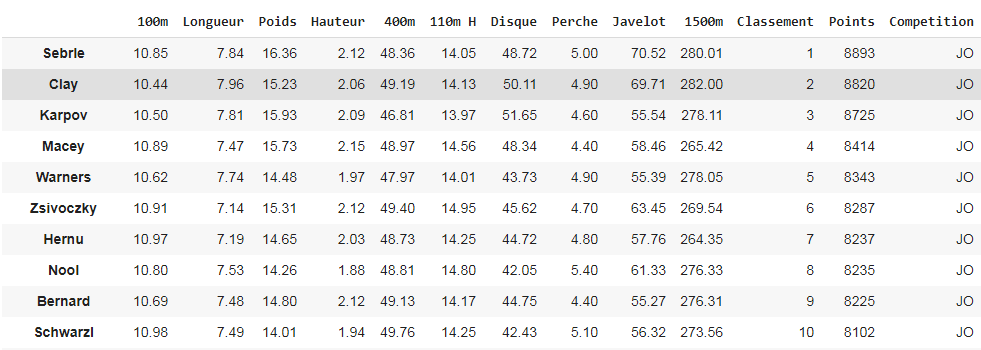
\includegraphics[width=\linewidth]{images/data_initials.png}
\end{figure}

On voit bien ici que les \textit{Variables} ne sont pas de même unité, alors on va d'abord les \underline{normalisées}. On peut confirmer que les \textit{Variables} sont bien normalisées quand elles sont asymptotiquement de moyenne nulle et de variance égale a un.

\begin{figure}[h!]
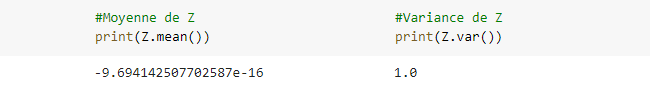
\includegraphics[width=\linewidth]{images/mean_variance.png}
\end{figure}

D'après ces résultats, les moyennes et les variances de nos \textit{Variables Normalisées} tendent bien vers 0 et 1 respectivement.
\newline

A partir d'ici, on va travailler avec les \textbf{Données Normalisées} 

\newpage

\subsection{Les variables explicatives}

Parfois, il y a des \textit{Variables} dont l'importance est néglisable par rapport aux autres, il est important de les reconnaitre ou même de les éliminer pour avoir une meilleur analyse des données. Les \textit{Variables} restantes issue de cette \underline{élimination} seront appelées \textit{Variables Explicatives}.
\newline

Il y a plusieurs méthodes pour retrouver les variables à éliminer, mais pour notre problème, on va utiliser la méthode du coudé, d'après \href{https://fr.qaz.wiki/wiki/Elbow_method_(clustering)}{Wikipedia - Méthode du coude (clustering)} 
\newline

\textit{La méthode du coude est une heuristique utilisée pour déterminer le nombre de clusters (Variables dans notre cas) dans un ensemble de données . La méthode consiste à tracer la} \textbf{variation expliquée} \textit{en fonction du nombre de clusters, et à choisir le coude de la courbe comme le nombre de clusters à utiliser. La même méthode peut être utilisée pour choisir le nombre de paramètres dans d'autres modèles basés sur les données, comme le nombre de composants principaux pour décrire un ensemble de données}
\newline

Pour ce faire, on a donc besoin des variation expliquée de chaque \textit{Variable} de notre données normalisées et de trace la courbe de la fonction f définie par:

\begin{equation*}
f(V_e)=\frac{(n-1)}{n}*V_e \quad , \; V_e \; est \; la  \; variance \; explicative.
\end{equation*}

\begin{figure}[h!]
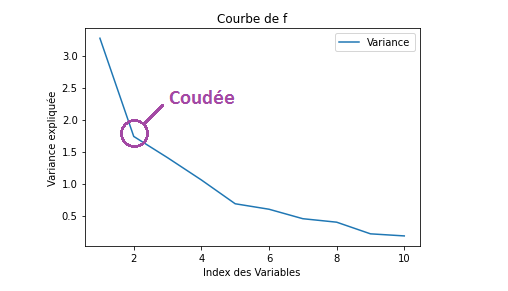
\includegraphics[width=\linewidth]{images/courbe_ve.png}
\end{figure}

D'après la graphe de la fonction - variance expliquée - on ne va donc retenir que les deux premières \textit{Variables} qui sont: la \textit{Variable 100m} et la \textit{Variables Longueur}.
\newline

\newpage

A partir de ces deux \textit{Variables}, on peut positionner les individus dans le plan. On a alors la figure suivante:

\begin{figure}[h!]
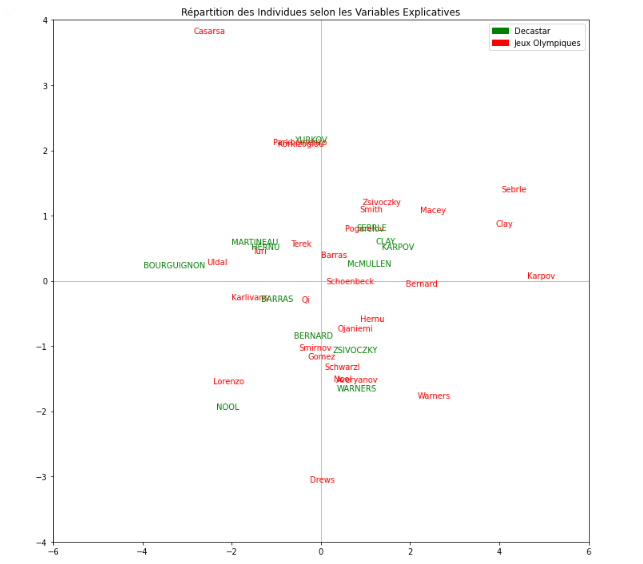
\includegraphics[width=\linewidth]{images/graph-plan.png}
\end{figure}

\subsubsection{Interpretation}

\underline{\textbf{Premier Axe}}: On peut remarquer du premier axe qu'elle departage les joueurs ayant un bon classement a ceux qui ont un mauvais classement pendant les deux competitions.
En effet, les joueurs \textbf{Karpov} et \textbf{Clay} qui sont le deuxieme et le troisieme dans le classement des Jeux Olympiques, et des Jeux de Decastar sont placés à droite dans la premier axe alors que le joueur \textbf{Uldal}, avant dernier du classement des JO et le joueur \textbf{Bourguignon}, dernier du classement de Decastar sont placés a gauche dans la premier axe. 
\newline
\underline{\textbf{Deuxieme Axe}}: On peut remarquer du deuxieme axe qu'elle departage les joueurs  

\begin{figure}[h!]
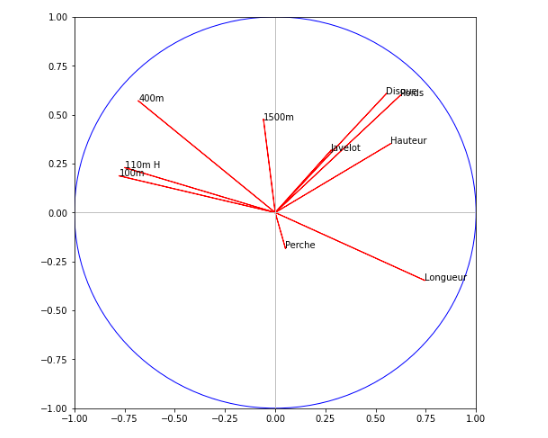
\includegraphics[width=\linewidth]{images/cercle_cor.png}
\end{figure}



\end{document}